\documentclass[12pt,a4paper]{article}

% --- Packages ---
\usepackage[utf8]{inputenc}
\usepackage[T1]{fontenc}
\usepackage{mathptmx}
\usepackage{amsmath,amssymb}
\usepackage{booktabs}
\usepackage{graphicx}
\graphicspath{{../output/figures/}}
\usepackage[margin=2.5cm]{geometry}
\usepackage[numbers,sort&compress]{natbib}
\usepackage[hidelinks]{hyperref}
\usepackage{caption}
\usepackage{xcolor}
\usepackage{float}

% --- Commands ---
\newcommand{\garcht}{GARCH(1,1)-\ensuremath{t}}
\newcommand{\garchn}{GARCH(1,1)-Normal}
\newcommand{\xbl}{XGBoost}
\newcommand{\hl}{\textsc{HighVol}}
\newcommand{\nor}{\textsc{Normal}}

\begin{document}

\title{Value-at-Risk Backtesting under Ex-Ante Regimes:\\
Evidence from Mexican FIBRAs}

\author{Author Name \\ \texttt{email@example.com}}
\date{\today}

\maketitle

\begin{abstract}
This paper evaluates Value-at-Risk (VaR) forecasting under ex-ante regime definitions in a data-constrained emerging REIT market. Using Mexican FIBRAs, we compare GARCH(1,1) models with Student-$t$ innovations against tuned XGBoost models across multiple assets. Under strictly out-of-sample, no-leakage conditions, GARCH-$t$ is associated with breach rates consistent with the nominal 5\% level, while XGBoost models produce breach rates around 12\% and are rejected by standard coverage tests. 

We find that this result is not explained by volatility forecast accuracy, as Diebold--Mariano tests fail to detect significant differences. The evidence is consistent with the interpretation that differences arise from tail modeling and finite-sample instability. A power analysis demonstrates that standard backtests have limited ability to detect moderate misspecification in short samples, implying that economically large errors may go statistically undetected.

The main contribution is to document a structural trade-off: ex-ante regime definitions eliminate look-ahead bias but severely reduce usable sample size, constraining statistical inference. In this setting, parsimonious parametric models are associated with better VaR calibration than flexible machine learning approaches. The findings are relevant for risk management in emerging markets, where data limitations are pervasive.
\end{abstract}

\section{Introduction}

Accurate Value-at-Risk (VaR) forecasting remains central to financial risk management and regulation. Standard backtesting procedures, such as unconditional and conditional coverage tests \citep{kupiec1995techniques,christoffersen1998evaluating}, are widely used but rely on sufficient sample sizes to provide meaningful inference. In practice, many applications—particularly in emerging markets—face severe data constraints.

At the same time, machine learning methods have gained prominence in financial prediction tasks, often demonstrating strong performance in large datasets \citep{gu2020empirical}. However, evidence on their effectiveness in small-sample, strictly out-of-sample risk forecasting remains limited. This raises an open question: does increased model flexibility translate into better risk calibration when data are scarce?

This paper addresses this question using Mexican FIBRAs (Fideicomisos de Infraestructura y Bienes Ra\'ices), the local equivalent of REITs. FIBRAs are a relatively recent financial innovation in Mexico, designed to channel investment into real estate through publicly traded vehicles \citep{fibras_cnbv,fibras_banxico}. While their institutional structure and market development have been documented \citep{fibras_amib,fibras_financialisation}, empirical evidence on their risk dynamics remains limited.

A key methodological contribution of this paper is the use of \textit{ex-ante} regime definitions. Unlike common ex-post classifications (e.g., crisis periods), our regime construction uses only information available at the forecast date, eliminating look-ahead bias. This design improves methodological validity but substantially reduces the usable sample.

Within this framework, we compare GARCH(1,1) models with Normal and Student-$t$ innovations against XGBoost-based volatility forecasts. The analysis focuses on VaR calibration rather than point prediction accuracy.

The contribution is threefold:

\begin{enumerate}
\item We document that ex-ante regime definitions impose a binding data constraint, creating a trade-off between methodological rigor and statistical power.
\item We show that, under these constraints, machine learning models are not associated with improved VaR calibration and tend to systematically underestimate tail risk in this setting.
\item We provide a power analysis of the Kupiec test, demonstrating that standard backtests have low power in realistic sample sizes.
\end{enumerate}

The results highlight the importance of aligning model choice with data availability. In this setting, when data are limited, a parsimonious parametric structure is associated with VaR calibration closer to the target coverage than more flexible alternatives.

\section{Data and Methodology}

\subsection{Data}

We use daily closing prices for FIBRATC14.MX, FUNO11.MX, FIBRAPL14.MX, the Mexican IPC Index (\^{}MXX), and EWW. The sample begins in 2018. Returns are computed as log-differences.

FIBRAs have grown significantly since their introduction in the early 2010s, becoming a key component of Mexican capital markets \citep{fibras_cnbv,fibras_banxico}. However, their relatively short history implies limited time-series depth. The heavy tails and volatility clustering documented in international REIT markets by \citet{cotter2012modelling} are also plausible features of FIBRA returns, and several other emerging-market REITs confront comparable data-scarcity constraints, which broadens the practical relevance of the present study without overstating its generalizability.

\subsection{Ex-Ante Regime Definition}

Regimes are defined ex ante using rolling realized volatility computed over a 20-trading-day window, lagged by one day to ensure no forward information enters the classification. Each day $t$ is labeled \hl{} if its trailing realized volatility exceeds the 90\textsuperscript{th} percentile of the distribution observed in a rolling 500-day backward-looking window ending at $t-1$, and \nor{} otherwise. This design replicates the information set of a real-time decision maker but is data-intensive: the initial 520 days are consumed by the regime construction alone. After intersecting with the rolling estimation requirements described below, the aligned out-of-sample window shrinks to 58 observations, of which only 4 fall in the high-volatility regime. The ex-ante approach therefore eliminates look-ahead bias at the cost of substantially reducing the effective sample, introducing a structural trade-off between methodological purity and statistical power that is central to the interpretation of the results.

\begin{figure}[H]
\centering
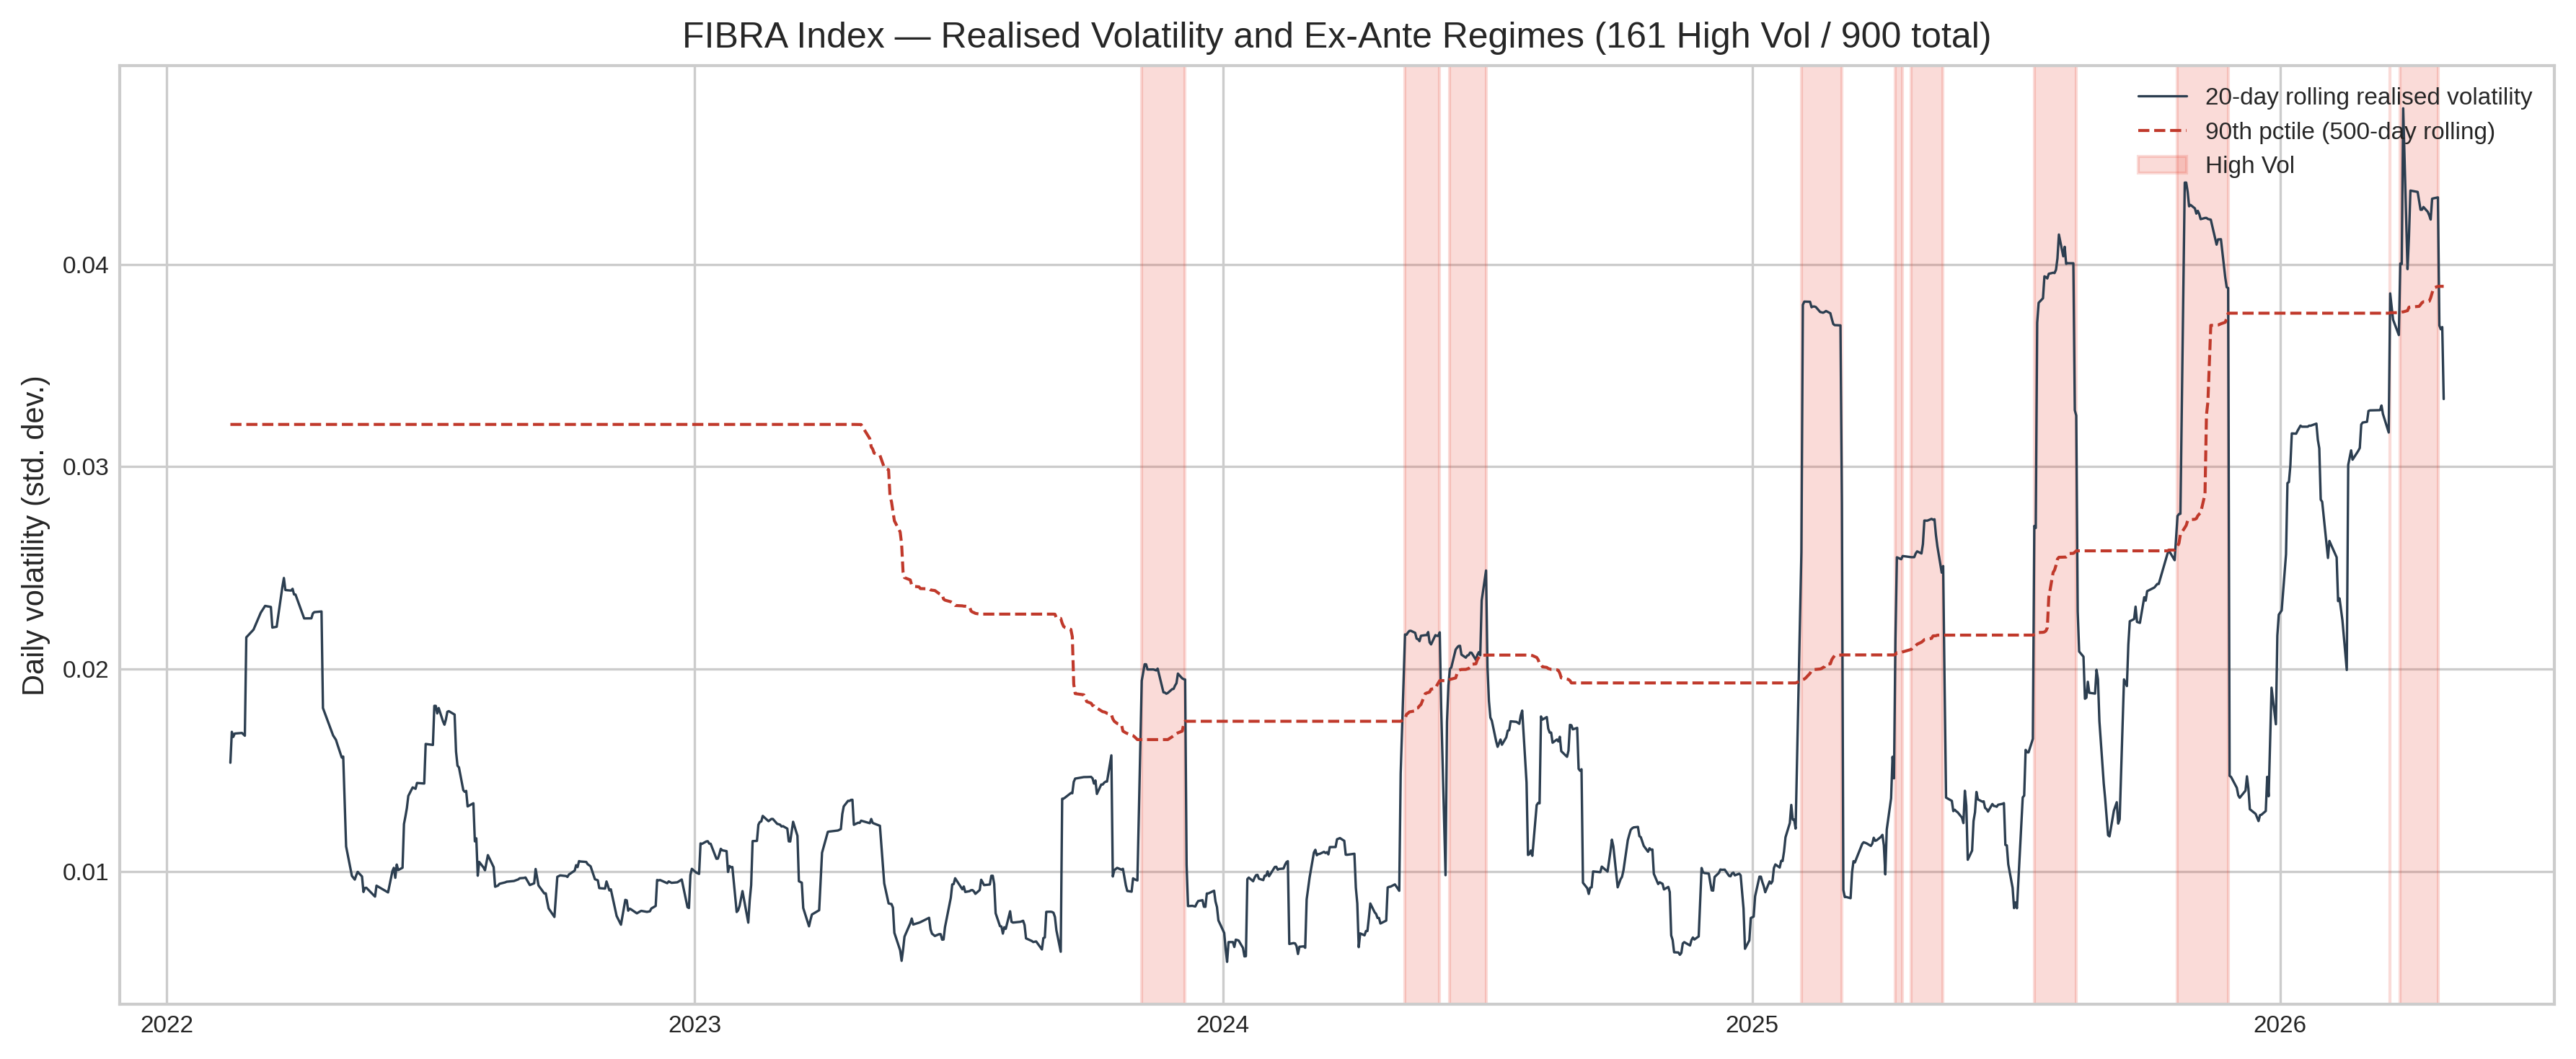
\includegraphics[width=0.95\textwidth]{fig1_volatility_regimes.png}
\caption{Realized volatility (20-day trailing standard deviation, solid line) with the 90\textsuperscript{th}-percentile threshold computed on a rolling 500-day window (dashed line). Shaded regions mark days classified as \hl{} ex ante; unshaded regions correspond to \nor{}. The figure shows the full available sample; after intersection with rolling estimation windows, the aligned out-of-sample subset contains 58 observations, of which only 4 occur during high-volatility periods.}
\label{fig:regimes}
\end{figure}

\subsection{Models}

We estimate:

\begin{itemize}
\item \garchn
\item \garcht
\item XGBoost (pure)
\item XGBoost with GARCH features (ensemble)
\end{itemize}

Models are trained on rolling windows of 125 observations and refitted periodically.

All XGBoost variants are tuned using temporal cross-validation (TimeSeriesSplit with three folds) to respect chronological order, combined with randomized hyperparameter search and early stopping. The tuning grid includes L2 regularization ($\lambda \in \{0.1, 1.0, 10.0\}$), shallow tree depths (2--4), and conservative learning rates (0.01--0.1), imposing a deliberately strong bias toward simpler solutions. The feature set for XGBoost is constructed entirely from lagged observables---including lagged absolute returns, squared returns, historical volatility, volume changes, and the USD/MXN exchange rate---so that the GARCH augmentation provided to the ensemble model is itself strictly ex ante. In contrast to the large-panel applications studied by \citet{gu2020empirical}, where tens of thousands of stock-month observations permit flexible models to learn stable patterns, the present setting involves at most a few hundred training returns per rolling window. Under these conditions even regularized tree ensembles can exhibit instability, and the finding that XGBoost underperforms in VaR calibration is specific to this data-scarce environment.

\subsection{VaR Backtesting}

VaR is computed at the 95\% level. Evaluation uses:

\begin{itemize}
\item Breach rates
\item Kupiec test \citep{kupiec1995techniques}
\item Christoffersen test \citep{christoffersen1998evaluating}
\item Expected Shortfall (Basel III) \citep{bcbs2019minimum}
\end{itemize}

\subsection{Finite-Sample Considerations}

The aligned out-of-sample period contains 58 observations. This reflects the interaction between regime construction and rolling estimation. The small sample size is a structural feature of the design.

\section{Results}

\subsection{VaR Calibration}

GARCH-$t$ produces breach rates consistent with the nominal 5\% (3 out of 58), whereas XGBoost-based models produce breach rates around 12\% (7 out of 58). The XGBoost models are rejected by the Kupiec test at conventional significance levels.

\begin{figure}[H]
\centering
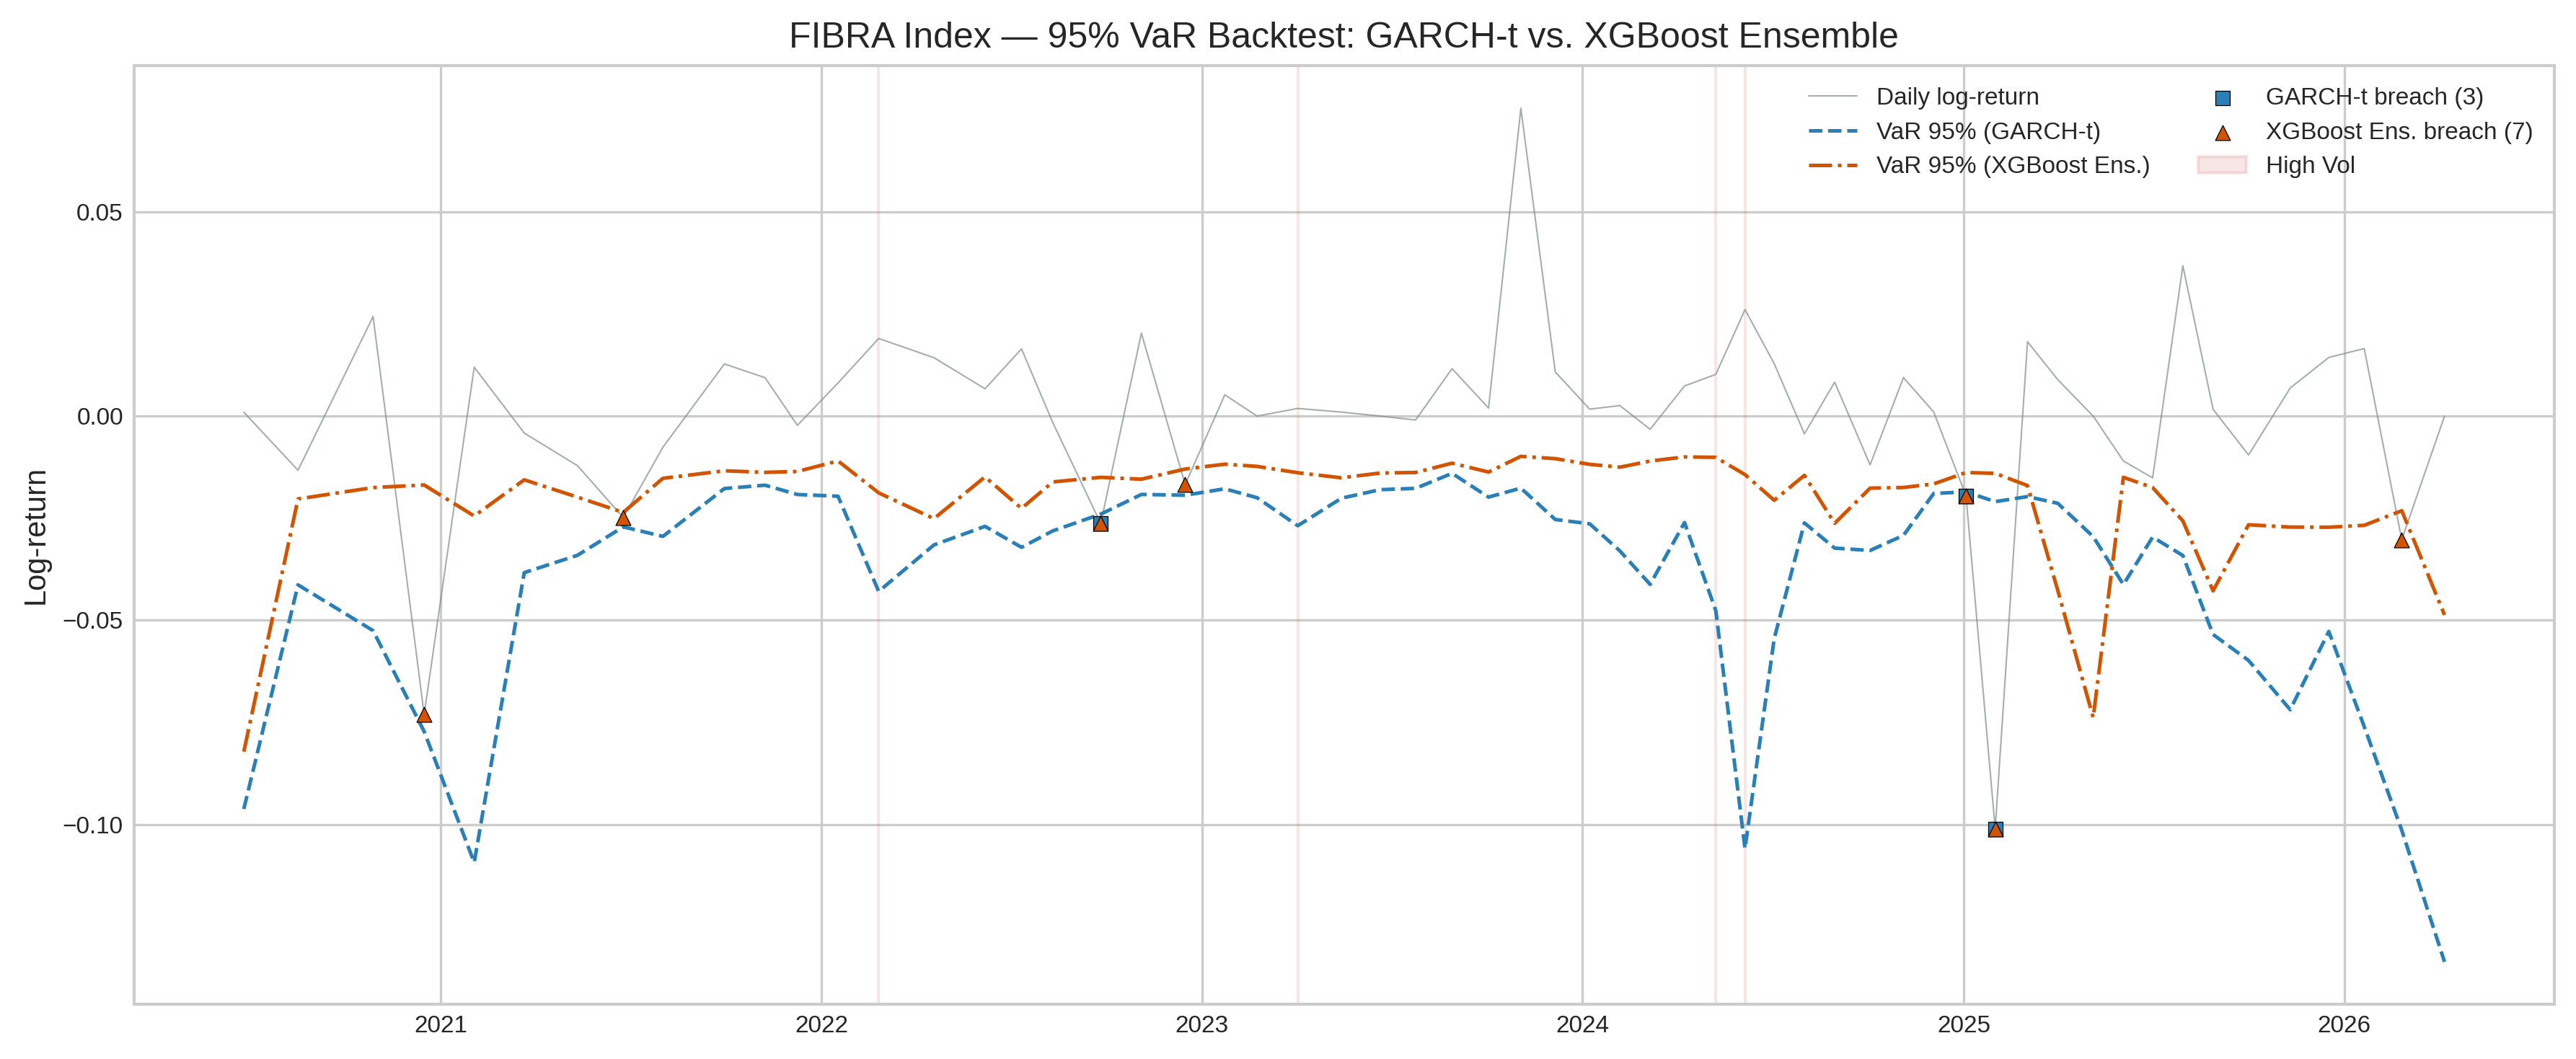
\includegraphics[width=0.95\textwidth]{fig2_var_violations.png}
\caption{Daily FIBRA log-returns (grey) with 95\% VaR bands for GARCH-$t$ (blue, dashed) and the XGBoost ensemble (orange, dash-dotted). VaR violations are marked with red circles. Ex-ante high-volatility regimes are shaded. The XGBoost ensemble produces systematically tighter VaR estimates, resulting in more frequent violations concentrated in volatile periods.}
\label{fig:violations}
\end{figure}

\subsection{Volatility Forecast Accuracy}

Diebold--Mariano tests do not detect significant differences at conventional levels. This suggests that similar MSE performance does not guarantee similar tail behavior.

\subsection{Power Analysis}

The Kupiec test has low power at $n=58$. To illustrate, under binomial reasoning, a Kupiec test at the 5\% level with a true breach rate of 10\% (double the nominal) achieves power below 0.20 when $n=58$; only deviations on the order of 15--20 percentage points are reliably detectable. Moderate misspecification is therefore unlikely to be detected statistically. The rejection of XGBoost thus reflects economically large errors, and conversely the non-rejection of GARCH-$t$ should not be interpreted as evidence of perfect calibration.

\begin{figure}[H]
\centering
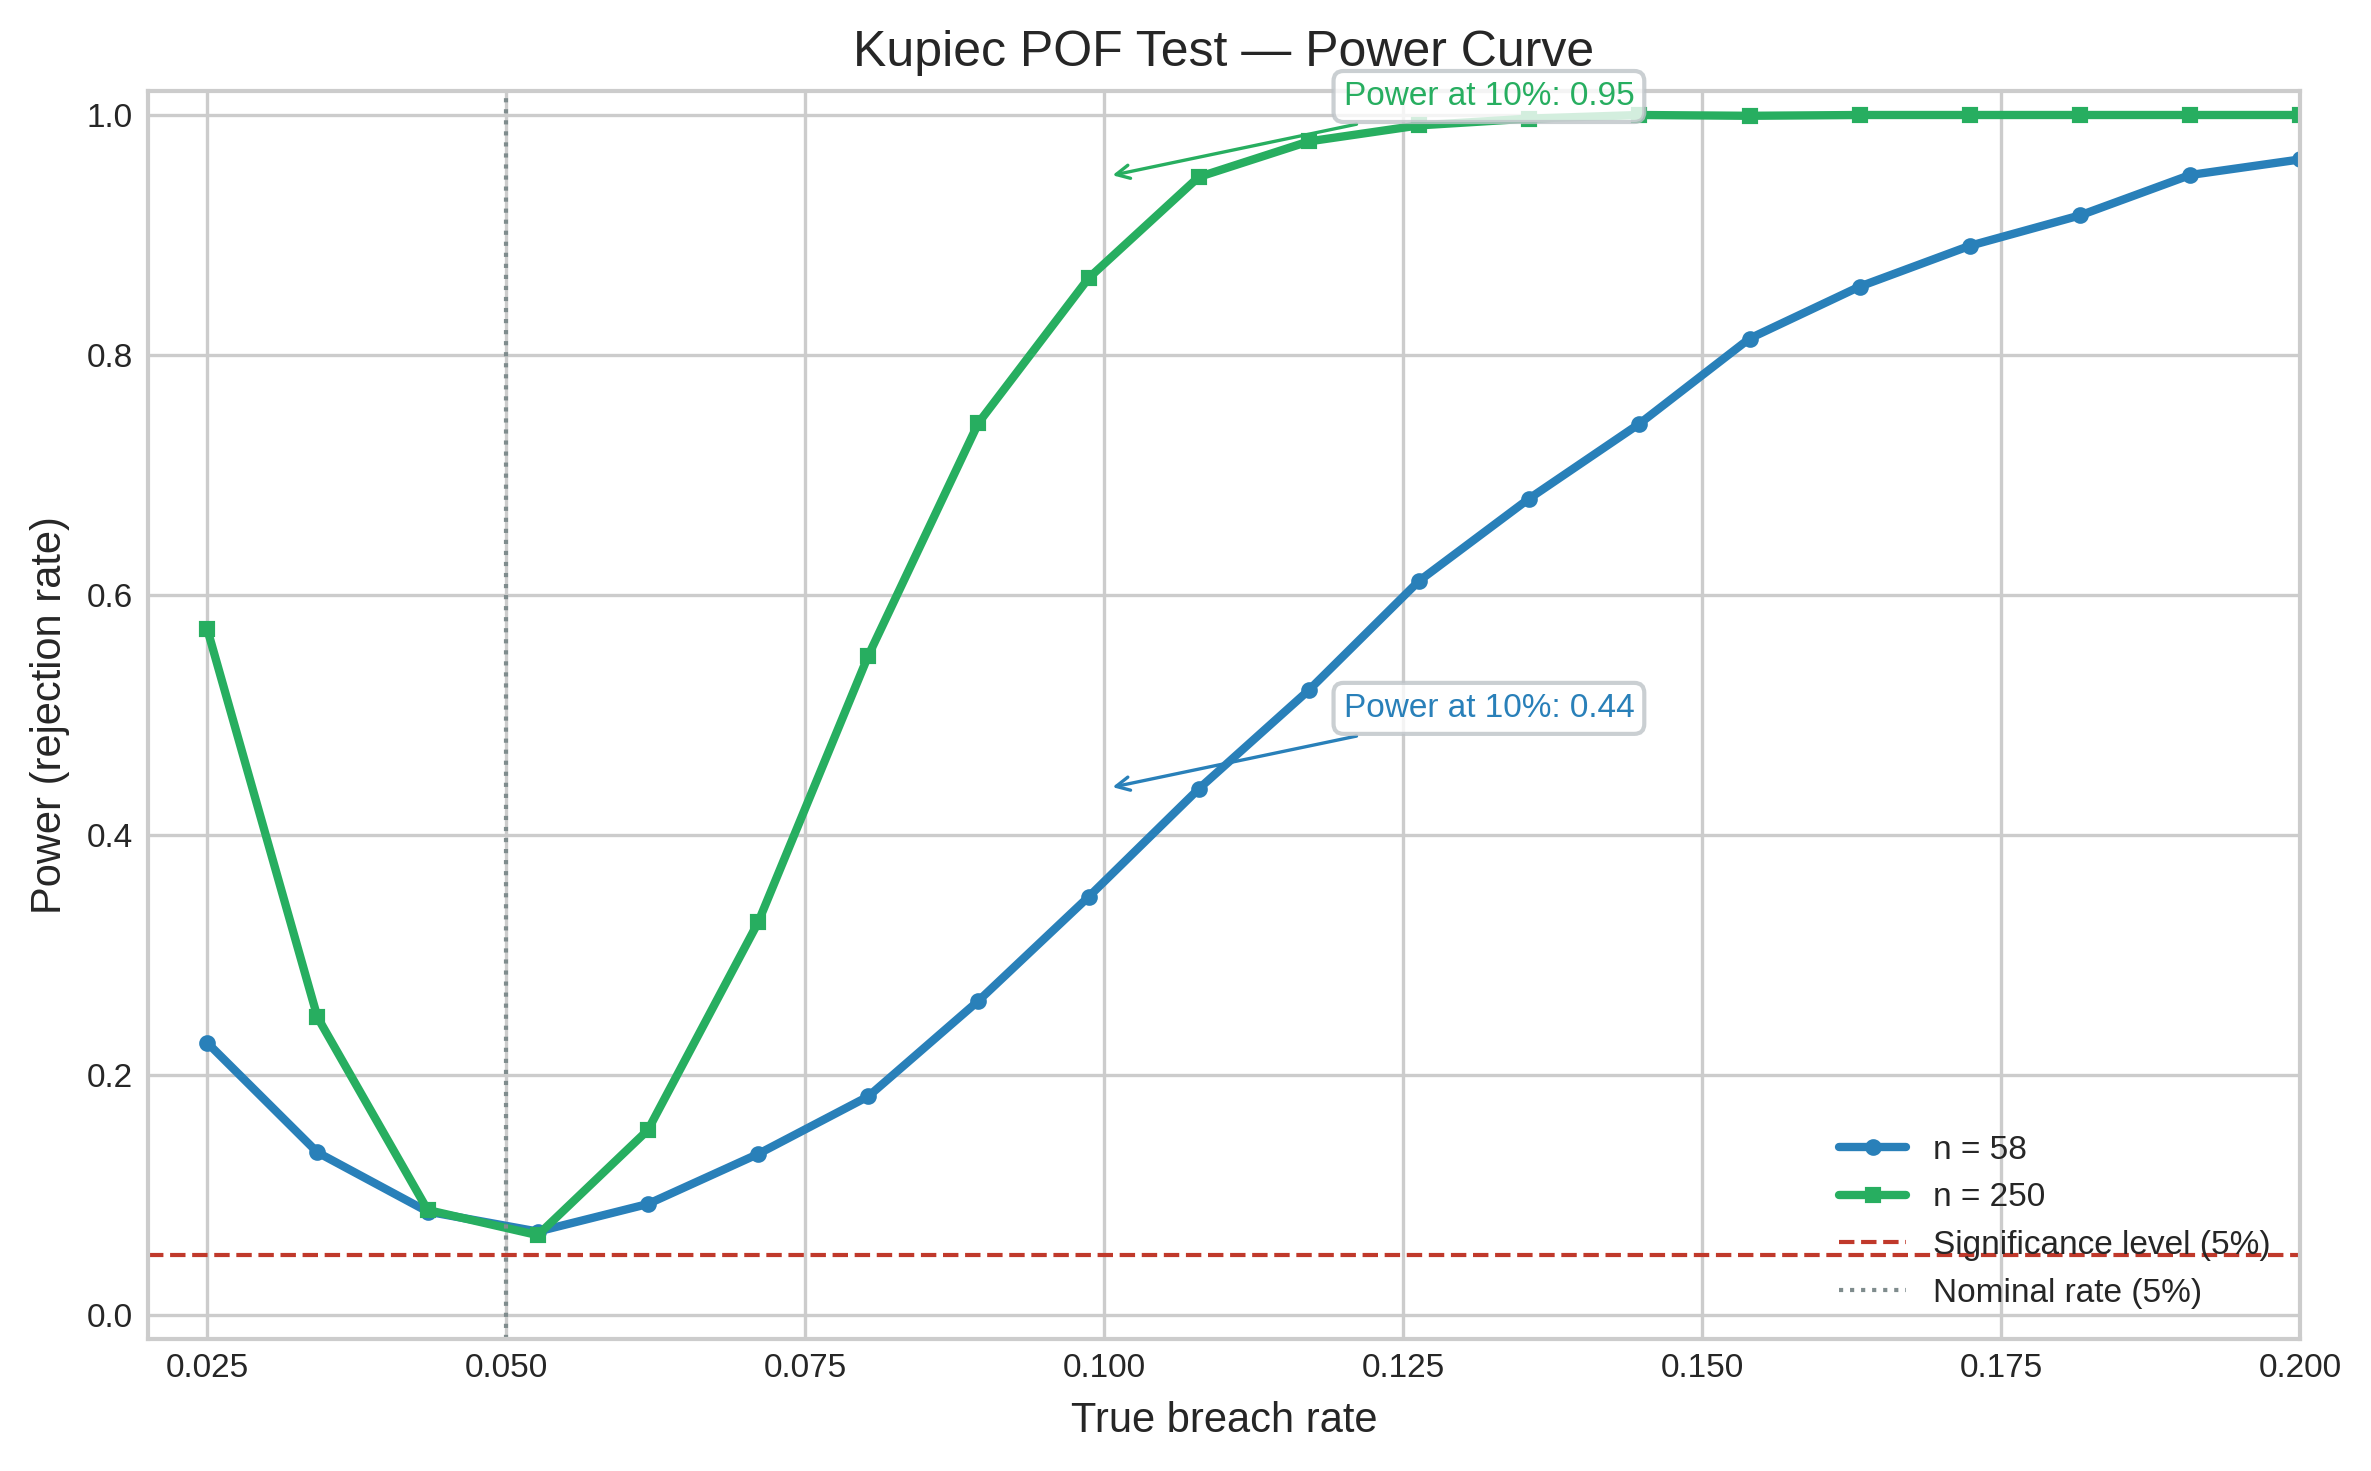
\includegraphics[width=0.85\textwidth]{fig3_power_curve.png}
\caption{Power curves of the Kupiec POF test for $n=58$ and $n=250$, estimated via 3\,000 binomial simulations at each true breach rate. The horizontal dashed line marks the 5\% significance level; the vertical dashed line indicates the nominal 5\% rate. At $n=58$, power remains below 0.50 even for breach rates three times the nominal level, whereas with $n=250$ the test achieves reasonable power for economically relevant deviations.}
\label{fig:power}
\end{figure}

\section{Discussion}

\subsection{Model Performance under Constraints}

The results suggest that, in this specific setting, greater model complexity does not translate into improved VaR calibration. The tail-aware parametric structure of GARCH-$t$ appears to act as an effective form of regularization for extreme quantiles in short samples.

\subsection{Why Machine Learning Underperforms}

Tree-based models trained with squared-error loss optimize central tendencies and, even with robustness-oriented hyperparameter choices, may not adequately represent the conditional tail behavior that VaR demands. In contrast, the Student-$t$ distribution directly accommodates heavy tails through its degrees-of-freedom parameter.

\subsection{Trade-Off between Rigor and Power}

Ex-ante regimes eliminate look-ahead bias but necessarily shrink the usable sample. This creates a binding constraint on the precision of empirical validation.

\section{Conclusion}

This paper studies VaR backtesting under realistic data constraints. The main finding is that, in the data-constrained environment of Mexican FIBRAs, simpler parametric models are associated with risk calibration that is more consistent with the nominal coverage level than flexible machine learning approaches.

More broadly, the results emphasize that methodological rigor and statistical power are jointly constrained in emerging markets. Future research should focus on larger samples, alternative ML architectures, and Expected Shortfall evaluation.

These findings are conditional on the specific time-series length of Mexican FIBRAs and the chosen ex-ante regime definition; while the broader lesson about backtesting design in data-scarce environments is likely to hold, the exact trade-offs will vary by market.

\section*{Data and Code Availability}

Code available at \url{https://github.com/example/fibras-var}.

\bibliographystyle{plainnat}
\bibliography{references}

\end{document}